% Suppress benign font substitution warnings from XeLaTeX/LuaLaTeX
\RequirePackage{silence}
\WarningFilter{latexfont}{Font shape}
\WarningFilter{latexfont}{Some font shapes}

\documentclass[conference]{IEEEtran}
\usepackage{cite}
\usepackage{amsmath,amssymb,amsfonts}
\usepackage{algorithmic}
\usepackage{graphicx}
\usepackage{textcomp}
\usepackage{xcolor}

\begin{document}

\title{The Extended SLM Combined Autoencoder of the PAPR Reduction Scheme in DCO-OFDM Systems}

\author{\IEEEauthorblockN{Lili Hao, Dongyi Wang, Yang Tao, Wenyong Cheng, Jing Li and Zehan Liu}
}

\maketitle

\begin{abstract}
End-to-end learning in optical communication systems is a promising technique to solve difficult communication problems, especially for peak to average power ratio (PAPR) reduction in orthogonal frequency division multiplexing (OFDM) systems. The less complex, highly adaptive hardware and advantages in the analysis of unknown or complex channels make deep learning a valid tool to improve system performance. In this paper, we propose an autoencoder network combined with extended selected mapping methods (ESLM-AE) to reduce the PAPR for the DC-biased optical OFDM system and to minimize the bit error rate (BER). The constellation mapping/de-mapping of the transmitted symbols and the phase factor of each subcarrier are acquired and optimized adaptively by training the autoencoder with a combined loss function. In the loss function, both the PAPR and BER performance are taken into account. The simulation results show that a significant PAPR reduction of more than 10 dB has been achieved by using the ESLM-AE scheme in terms of the complementary cumulative distribution function. Furthermore, the proposed scheme exhibits better BER performance compared to the standard PAPR reduction methods.
\end{abstract}

\begin{IEEEkeywords}
orthogonal frequency division multiplexing; autoencoder; end-to-end learning; peak-to-average power ratio
\end{IEEEkeywords}

\section{Introduction}
Visible light communication (VLC) based on light emitting diodes (LEDs) is a promising technology for indoor wireless access \cite{b1}\cite{b2}\cite{b3}. To overcome the multipath distortion caused by reflections from different sources inside a room and enhance the communication efficiency, the optical orthogonal frequency division multiplexing (OFDM) has been widely adopted in VLC systems \cite{b4}\cite{b5}\cite{b6}\cite{b7}. However, the high peak to average power ratio (PAPR) associated with the OFDM signals is one of the main limitations for VLC systems due to the constraints on the average radiated optical power and the limited dynamic range of the front-end devices, like digital to analog converters and power amplifiers \cite{b8}. High PAPR makes the VLC system more susceptible to non-linear distortions and consequently drastically degrade the system's performance \cite{b9}\cite{b10}\cite{b11}.

Several PAPR reduction techniques for DC-biased optical orthogonal frequency division multiplexing (DCO-OFDM) systems have been investigated in the literature. The authors proposed a genetic algorithm and peak-value optimization algorithm \cite{b12} to mitigate the high PAPR in VLC systems with lower complexity. The study in \cite{b13} used a semidefinite relaxation method for tone injection to reduce the PAPR for the DCO-OFDM. The branch and bound method \cite{b14} and tone reservation method \cite{b15} were also proposed to lower the impact of the high PAPR in VLC systems. Nevertheless, these methods reduce the PAPR at the sacrifice of computational complexity and channel resources. Moreover, the authors in \cite{b16} introduced a pilot-assisted approach to achieve improved PAPR performance over the select mapping scheme for high-level constellations. However, it resulted in a data rate loss according to the density of pilot symbols. In addition, a subcarrier grouping scheme for the OFDM-based VLC system \cite{b17} is proposed to reduce the PAPR, but at a lower signal-to-noise ratio (SNR) the bit error rate (BER) performance was inferior to that of DCO-OFDM.

To mitigate the effects of these limitations, deep learning offers an efficient option for its good generalization properties with flexible modeling and learning capabilities. Deep learning is a promising technique to solve difficult communication problems \cite{b18} for its minimal complicity, adaptive hardware and robustness in the analysis of the unknown or complex channels. Use of deep learning methods to solve difficult communication problems has been reported and has demonstrated better performances than conventional communication methods in the end-to-end learning of encoding and decoding application \cite{b19}. Another approach reported in \cite{b20} is the end-to-end learning of a prototype consisting of two software-defined radios that communicate over an actual wireless channel. Deep learning techniques for channel estimation and symbol detection in an end-to-end manner \cite{b21} are investigated which have wide application in many communication systems. Among them, a special network architecture named autoencoder (AE) which is usually used for denoising corrupted data is suitable to dealing with the non-linear distortions caused by the high PAPR \cite{b22}. It optimizes reconstruction loss through a series of representations typically using a mean squared error objective and a stochastic gradient descent solver to find network weights achieving an effective regression \cite{b23}. An AE-based system \cite{b24} that was solely composed of Neural Networks communicating over-the-air was extended in the OFDM scheme. Kim and Cho \cite{b22} proposed a PAPR-reducing network and discussed the PAPR behavior in the RF system. Sohn and Kim \cite{b25}\cite{b26} applied an artificial neural network to reduce the complexity in solving the PAPR reduction problem. However, the focus of these studies was limited to the clipping and filtering technique and active constellation extension signals, which may not acquire better performance than conventional methods when extended to optical OFDM systems.

A novel deep neural network combined with extended Selected Mapping (ESLM), namely ESLM-AE, is proposed in this paper to mitigate the high PAPR issue of DCO-OFDM signals. It uses an AE structure to represent the constellation mapping and de-mapping of the transmitted symbols. In the network, the ESLM method is added after the constellation mapping to reduce the high PAPR of the DCO-OFDM system. By designing the loss function of neural network and considering both the BER and PAPR performance, autoencoder and SLM can be combined organically. Further, the phase factor of SLM can be determined and optimized accordingly in the network training process. Thus, it is expected that the proposed ESLM-AE method is more efficient in reducing the PAPR without deterioration of the BER performance.

The remainder of this paper is organized as follows. Section II-A gives an overview of the DCO-OFDM system model. Section II-B presents the detailed architecture of the proposed ESLM-AE scheme. Section III contains the simulation results and a discussion of the proposed scheme compared to the standard methods in different channels. Finally, conclusions are reported in Section IV.

\section{Methods}
\subsection{An Overview of the DCO-OFDM System Model}
Fig.~\ref{fig1} shows an overview of the DCO-OFDM transmitter and receiver structure based on the proposed ESLM-AE scheme. Different from the conventional DCO-OFDM system, an AE is applied in the whole model. AE is a special neural network which can represent the mapping from the input to itself because of universal approximation theorem \cite{b27}\cite{b28}. The neurons in the hidden layer of autoencoder can be considered as a coding representation of input.

\begin{figure}[htbp]
\centerline{
\includegraphics[width=\linewidth]{Figures/1.png}}
\caption{An overview of the DC-biased optical orthogonal frequency division multiplexing (DCO-OFDM) system with the autoencoder network combined with extended selected mapping methods (ESLM-AE) structure.}
\label{fig1}
\end{figure}

In our scheme, the input signals are firstly fed into the encoder and phase rotator modules before Hermitian symmetry and inverse fast Fourier transform (IFFT) to get the in-phase and quadrature (I-Q) constellation mapping and generate the alternative output sequence. The outputs of IFFT are then converted into unipolar by adding DC bias and clipping. Signal clipping is performed in order to fit the real time-domain OFDM symbols into a limited range of the LED. In the optical channel, the transmitted signals are influenced by the noise sources in a real scenario. At the receiver side, phase recovery and the decoder part aim to recover the distorted signals. The network can be trained with the lowest PAPR and BER.

It is assumed that the OFDM signal is transformed by $2N$ subcarriers. Let $x$, $f(x)$ and $g(x)$ be the input of encoder, encoder, and decoder of the AE, respectively. According to the DCO-OFDM system, the transmitted data stream is mapped into complex-value symbols. As shown in Fig.~\ref{fig1}, after serial to parallel conversion, the input data sequence is divided into $2N$ messages $x$, where $x = [x_0, x_1, \dots , x_{2N-1}]^T$. Then $x$ is mapped into I-Q constellation according to the encoder part which will be detailed discussed in Section II-B. We define the output of the encoder $X = f(x)$, where $X \in \Re^{2N}$ consists of $2N$ real values and among them pairwise combination in a certain order forms $N$ complex symbols $A$, $A = [A_0, A_1, \dots , A_{N-1}]^T$, $A \in \mathbb{C}^N$.

However, the classic AE is only designed to minimize the BER. In practice, the transceiver usually suffers from a high PAPR. To mitigate the high PAPR, each $A_k$, $k = 0, 1, \dots , N - 1$, is multiplied by a phase factor $a_k$ which can be expressed as $A'_k = A_k \cdot a_k$, where $a_k = e^{j\psi_k}$ and $\psi_k \in [0, 2\pi)$ \cite{b29}. For the VLC-OFDM system, the intensity modulation requires the transmitted signals of the LED to be nonnegative and real-valued \cite{b5}. Thus, Hermitian symmetry is imposed on $A'_k$ to form the frequency domain OFDM symbols $S = [A'_0, A'_1, \dots , A'_{N-1}, A_{N-2}^*, \dots , A_{1}^*]$ and the DC components are $A'_0 = A'_{N-1} = 0$. This results in a $2N$-point IFFT output of the OFDM symbols. Subsequently the time domain OFDM signal can be obtained by feeding $S(k)$, $k = 0, 1, \dots , 2N - 1$, into an inverse discrete Fourier transform using Equation (\ref{eq1}).

\begin{equation}
s(n) = \frac{1}{\sqrt{2N}} \sum_{k=0}^{2N-1} S(k)e^{j2\pi nk/2N},
\label{eq1}
\end{equation}

where $n = 0, 1, \dots , 2N - 1$.
Consequently, the PAPR of the DCO-OFDM signal is calculated using Equation (\ref{eq2}).

\begin{equation}
PAPR\{s(n)\} = \frac{\max_{0\leq n\leq 2N-1}|s(n)|^2}{E\left[|s(n)|^2\right]} ,
\label{eq2}
\end{equation}

where $n = 0, 1, \dots , 2N - 1$. When the high amplitudes of different subcarriers with the same phase appear at the same time, the high PAPR will appear. Complementary cumulative distribution function (CCDF) is used to denote the probability that the PAPR of signals will exceed a given threshold value, $PAPR_0$, i.e., $CCDF = \text{Pr}(PAPR > PAPR_0)$.

After the parallel to serial conversion and adding a cyclic prefix (CP), the DC bias and clipping are added to the time-domain discrete signals $s(n)$ to ensure all the signal amplitudes are nonnegative. In VLC systems, the transmitted signal has to be constrained in the linear range due to the nonlinear characteristics of LED \cite{b30}. Accordingly, $s(n)$ is subjected to amplitude clipping at given upper ($\xi_{upper}$) and lower ($\xi_{lower}$) levels before fed into LED. Assume the linear range of LED is $[0, 2\xi_{upper}]$ and the symmetric clipped signal of $s(n)$ is given in Equation (\ref{eq3}) \cite{b31}.

\begin{equation}
x_{Clipped}(n) =
\begin{cases}
\xi_{upper}, & s(n) > \xi_{upper} \\
s(n), & \xi_{lower} \leq s(n) \leq \xi_{upper} , \\
\xi_{lower}, & s(n) < \xi_{lower}
\end{cases}
\label{eq3}
\end{equation}

where $n = 0, 1, \dots , 2N - 1$. We define $\xi_{upper} = -\xi_{lower} = \gamma \sqrt{E[|s(n)|^2]}$ and $\gamma$ is referred to the clipping ratio. To assure a steady light intensity and maximize the modulation depth, the DC bias is set as $B_{DC} = \xi_{upper}$, Then the DCO-OFDM signals fed into LED are expressed as Equation (\ref{eq4}).

\begin{equation}
x_{DCO}(n) = x_{Clipped}(n) + \mathbf{B}_{DC} =
\begin{cases}
2\xi_{upper}, & s(n) > \xi_{upper} \\
s(n) + \xi_{upper}, & -\xi_{upper} \leq s(n) \leq \xi_{upper} , \\
0, & s(n) < -\xi_{upper}
\end{cases}
\label{eq4}
\end{equation}

where $n = 0, 1, \dots , 2N - 1$. Essentially, clipping noise will degrade the performance of the DCO-OFDM system due to the non-linear distortion.

Subsequently the unipolar signal drives the LED to converts the electrical signals to the optical signals. In the optical channel, the line-of-sight (LOS) links are assumed to dominate over all multipath components from the wall and ceiling reflections. The received signal is influenced by the noise sources in a real scenario. The dominant noise source in an indoor wireless optical channel is the ambient light induced shot noise \cite{b32}, which is modeled as the additive white Gaussian noise (AWGN) given by $Z = [Z_0, Z_1, \dots , Z_{2N-1}]^T$. It has been considered that there is no additional clipping introduced by the photodetector (PD). Thus, after converting the optical signals to electrical signals using PD, the received signal, $y = [y_0, y_1, \dots , y_{2N-1}]^T$ can be computed using Equation (\ref{eq5}).

\begin{equation}
y = x_{DCO} \otimes q + Z,
\label{eq5}
\end{equation}

where $x_{DCO}$ is the vector of DCO-OFDM signal $x_{DCO}(n)$, $q$ is the channel response, $Z$ is AWGN with zero mean and variance of $\sigma_Z^2$ and $\otimes$ denotes the convolution operation. We assume that the channel state information is perfectly known in advance.

Then a reverse process can be implemented to demodulate the data. After removing the DC bias, the corresponding vector $y$ passes through the fast Fourier transform (FFT) operation. A simplified representation of the output $Y$ is shown in Equation (\ref{eq6}).

\begin{equation}
Y = FFT\{Q \circ IFFT[f(x)] + \varepsilon\},
\label{eq6}
\end{equation}

where $Q$ denotes the effects of the optical channel and $\varepsilon$ is the noise at the receiver. Finally $Y$ is transformed to the decoder $g(Y)$, which functions as the constellation mapper to get the recovered symbol $\hat{x}$.

\subsection{The ESLM-AE PAPR Reduction Scheme}
The neural network, which is an important statistic tool, can be used for describing the relationship between the input and the output. Its parameters can be determined automatically using backpropagation given a particular loss function. The proposed ESLM-AE uses an AE structure combined with ESLM method to mitigate the high PAPR issue of DCO-OFDM signals.

\subsubsection{Autoencoder Network}
In our scheme, an AE network is applied to the DCO-OFDM system to optimize the end-to-end performance.

Usually a feedforward neural network (NN) with $L$ layers describes a mapping $f(r_0; \theta) : \mathbb{R}^{N_0} \mapsto \mathbb{R}^{N_L}$ of an input vector $r_0 \in \mathbb{R}^{N_0}$ to an output vector $r_L \in \mathbb{R}^{N_L}$ through $L$ iterative processing steps \cite{b33}:

\begin{equation}
r_\ell = f_\ell(r_{\ell-1}; \theta_\ell), \quad \ell = 1, \dots , L
\label{eq7}
\end{equation}

Where $f_\ell(r_{\ell-1}; \theta_\ell) : \mathbb{R}^{N_{\ell-1}} \mapsto \mathbb{R}^{N_\ell}$ is the mapping carried out by the $\ell$th layer and $\theta = \{\theta_1, \dots , \theta_L\}$ is used to denote the set of all parameters of the network. The $\ell$th layer is called dense or fully-connected (FC) layer if $f_\ell(r_{\ell-1}; \theta_\ell)$ has the form

\begin{equation}
f_\ell(r_{\ell-1}; \theta_\ell) = \rho(W_\ell r_{\ell-1} + b_\ell),
\label{eq8}
\end{equation}

Where $W_\ell \in \mathbb{R}^{N_\ell \times N_{\ell-1}}$, $b_\ell \in \mathbb{R}^{N_\ell}$, are the weights and bias for the $\ell$th layer respectively. $\rho(\cdot)$ is an activation function and the set of parameters for this layer is $\theta_\ell = \{W_\ell, b_\ell\}$.

For the classic AE, its expected output is the input, which is different from other neural networks. Therefore, the AE can be trained from scratch without supervision, and a multilayer network can represent a mapping from the input to the expected output, identity as the input. The AE has been applied in many communication fields such as channel encoding and decoding, channel compensation and modulation recognition \cite{b22}\cite{b23}\cite{b24}.

A brief illustration of the proposed AE system is shown in Fig.~\ref{fig2} \cite{b20}. The transmitter part is called the encoder and it maps the input signals into the I-Q constellation. We assume both encoder and decoder are composed of $L_f = L_g = 3$ sub-blocks. Each of the sub-blocks is composed of dense layer, batch normalization (Batchnorm), activation function and dropout.

\begin{figure}[htbp]
\centerline{
\includegraphics[width=\linewidth]{Figures/2.png}}
\caption{Illustration of the proposed autoencoder system.}
\label{fig2}
\end{figure}

Let $r^f_\ell$ be the input of the $\ell$th dense layer of the encoder and the output can be expressed as $h^f_\ell = W^f_\ell r^f_\ell + b^f_\ell$, where $W^f_\ell$ and $b^f_\ell$ are the weights and bias for the $\ell$th layer. The output of each dense layer passes through the batch normalization (Batchnorm) layer to minimize the internal covariate shift.

Then the normalized value is fed into the activation function to make the data features nonlinear. The activation functions used in our scheme are the rectifier linear unit (ReLU) \cite{b33} and sigmoid \cite{b34}. In the encoder part the activation function used in each of the sub-blocks is ReLU.

Finally, dropout is used for addressing the overfitting problem for the proposed AE network, which has large number of parameters. The key idea is to randomly drop units from the neural network during training, which significantly reduces overfitting and gives major improvements over other regularization methods \cite{b35}.

As is shown in Fig.~\ref{fig2}, the output of the encoder is then transmitted to the simulated channel and decoder. Decoder has a similar structure as the encoder network. The only difference is the activation function of the last sub-block is sigmoid. It aims to recover the original binary information from the distorted signal after the complicated channel transmission.

Mathematically, the output of the encoder can be expressed as Equation (\ref{eq9}) \cite{b22}.

\begin{equation}
X = f(x) = \rho_{L_f} \left( \left. W_{L_f}^f \rho_{L_f-1} \left( \dots \rho_1 \left( \left. W_1^f x + b_1^f \right|_{norm} \right) \dots \right) + b_{L_f}^f \right|_{norm} \right),
\label{eq9}
\end{equation}

where $W_{L_f}^f$ and $b_{L_f}^f$ are the weights and bias for the $L_f$th dense layer of the encoder respectively.

Similarly, the output of the decoder can be expressed as Equation (\ref{eq10}).

\begin{equation}
\hat{x} = g(Y) = \rho_{L_g} \left( \left. W_{L_g}^g \rho_{L_g-1} \left( \dots \rho_1 \left( \left. W_1^g Y + b_1^g \right|_{norm} \right) \dots \right) + b_{L_g}^g \right|_{norm} \right),
\label{eq10}
\end{equation}

where $W_{L_g}^g$ and $b_{L_g}^g$ are the weights and bias for the $L_g$th dense layer of the decoder respectively.

As mentioned, the noise channel could distort the signal during the transmission. The AE aims to find an adequate encoding and decoding strategy to eliminate the complex optical channel and noise interference. To achieve the objective, the first network loss function can be set as the reconstruction error given in Equation (\ref{eq11}).

\begin{equation}
Loss_1(x, \hat{x}) = \|x - \hat{x}\|^2,
\label{eq11}
\end{equation}

For the training of the AE, the stochastic gradient descent (SGD) \cite{b33} optimization method is popular used which starts with some random initial values of $\theta = \theta_0$ and update $\theta$ iteratively as

\begin{equation}
\theta_{t+1} = \theta_t - \lambda \nabla_\theta Loss_1(x, \hat{x}),
\label{eq12}
\end{equation}

where $\lambda > 0$ is the learning rate, $\theta$ denotes parameters of the AE and $\nabla_\theta$ denotes the Gradient operation $\frac{\partial Loss_1(x, \hat{x})}{\partial \theta}$.

\subsubsection{Extended Selected Mapping Technique}
For the DCO-OFDM, a high signal peak value implies a need for a large DC bias that causes serious degradation of the system's power efficiency. Therefore, inspired by SLM, a reduction scheme, named extended Selected Mapping method is given in this section.

The Selected Mapping (SLM) method is one popular scheme to reduce the PAPR, because it is simple to implement without introducing any distortion to the signal and it can be used with any subcarrier number and modulation style \cite{b36}. The principle is that $U$ copies of the complex data vector $C^u = [C^u_0, C^u_1, \dots , C^u_{N-1}]$ are multiplied by $u$ distinct phase vectors $B^u = [B^u_0, B^u_1, \dots , B^u_{N-1}]$, $u = 1, 2, \dots , U$. The corresponding time domain data vector after IFFT is shown in Equation (\ref{eq13}).

\begin{equation}
c_n^u = IFFT\{C_k^u \cdot B_k^u\},
\label{eq13}
\end{equation}

where $n = 0, 1, \dots , N - 1$.

The objective of the SLM technique is to determine the transmitted $c_n^u$ using Equation (\ref{eq14}) \cite{b29}.

\begin{equation}
\min_{(B^u)} \left( \frac{\max \left\{|c_n^u|^2, n = 0, 1, \dots N - 1\right\} }{\frac{1}{N} \sum_{n=0}^{N-1} |c_n^u|^2} \right),
\label{eq14}
\end{equation}

To improve the PAPR reduction performance of the SLM scheme, the SLM technique requires an increase in the number of phase sequences. However, the computational complexity of the SLM scheme linearly increases as the number of phase sequences increases. The alternative method is an extensive search for the optimal sequence that achieves the minimum PAPR. Consequently, in the SLM, the PAPR reduction is primarily dependent on the chosen phase sequence candidates \cite{b37}.

In this paper, we extended the SLM technique to AE to get the adaptive phase sequence shown in Fig.~\ref{fig3}. Each phase factor $a_k$ of $A_k$ no longer needs to be artificially arranged since it can be trained and continuously optimized in the deep learning network. Simultaneously, in the test, once the phase sequence is determined, the calculation of the IFFT is needed only once.

\begin{figure}[htbp]
\centerline{
\includegraphics[width=\linewidth]{Figures/3.png}}
\caption{Partial block diagram of an OFDM transmitter with the extended Selected Mapping (SLM) technique.}
\label{fig3}
\end{figure}

In our proposed scheme, the network is trained to reduce the PAPR without reducing the BER performance \cite{b38}. Consequently, two distinct factors must be taken into the account at the same time. To reduce PAPR value, we define the second loss component $Loss_2(x)$ which is given as Equation (\ref{eq15}).

\begin{equation}
Loss_2(x) = PAPR\{s(n)\},
\label{eq15}
\end{equation}

Based on simulation, the $Loss_2(x)$ is helpful to reduce the high PAPR and lower distortion will in turn improve the BER performance in the training process.

Considering the two factors, we use a hyperparameter $\eta$ to balance the two different loss components. Thus, the total loss function can be expressed in Equation (\ref{eq16}).

\begin{equation}
Loss(x, \hat{x}) = Loss_1(x, \hat{x}) + \eta Loss_2(x),
\label{eq16}
\end{equation}

Notice that each phase factor $a_k$ of $A_k$ can be trained in terms of $\frac{\partial Loss}{\partial a_k}$ based on the propagation algorithm \cite{b39}.

\section{Results and Discussion}
In this section, simulation results are presented to demonstrate the PAPR and BER performances of the proposed scheme in different channels. The parameters of the network are shown in Table \ref{tab1}.

\begin{table}[htbp]
\caption{Parameters of the proposed network.}
\begin{center}
\begin{tabular}{|l|c|}
\hline
\textbf{Parameter} & \textbf{Value} \\
\hline
Transmitter (TX) dimensions & \\
Input & 128 \\
Dense (ReLU) & 2048 \\
Dense (ReLU) & 2048 \\
Dense (ReLU) & 128 \\
\hline
Receiver (RX) dimensions & \\
Input & 128 \\
Dense (ReLU) & 2048 \\
Dense (ReLU) & 2048 \\
Dense (sigmoid) & 128 \\
\hline
Optimizer & SGD with Adam \cite{b40} \\
Learning rate $\lambda$ & 0.0001 \\
Batch size & 32 \\
Weight parameter $\eta$ & 0.01 \\
Dropout probability & 0.1 \\
Number of subcarriers & 128 \\
Length of cyclic prefix & 32 \\
\hline
\end{tabular}
\label{tab1}
\end{center}
\end{table}

\begin{table}[htbp]
\caption{Results Comparison of the training set, validation set and test set.}
\begin{center}
\begin{tabular}{|l|c|c|c|}
\hline
\textbf{Results} & \textbf{Training set} & \textbf{Validation set} & \textbf{Test set} \\
\hline
Average PAPR & 2.0198 & 2.0499 & 2.0439 \\
BER & 0.0003976 & 0.0004077 & 0.0004059 \\
\hline
\end{tabular}
\label{tab2}
\end{center}
\end{table}

\subsection{PAPR Comparison}
First, we evaluated the PAPR performance of the presented system compared to AE, SLM, DCO-OFDM with different clipping ratio $\gamma$ and the DCO-OFDM with no PAPR reduction scheme. CCDF curves are presented to illustrate the PAPR comparison results depicted in Fig.~\ref{fig4}. It can be observed from Fig.~\ref{fig4} that the PAPR of the proposed ESLM-AE method outperforms other methods with a PAPR reduction gain of 10.8 dB compared to DCO-OFDM, while the SLM $U = 128$ gives the least PAPR reduction gain of 4.9 dB.

\begin{figure}[htbp]
\centerline{
\includegraphics[width=\linewidth]{Figures/4.png}}
\caption{Complementary cumulative distribution function (CCDF) of peak to average power ratio (PAPR) comparison of ESLM-AE, Autoencoder, clipped DCO-OFDM, DCO-OFDM and SLM. The clipping ratios, $\gamma$, used for ESLM-AE and Autoencoder is 1.5.}
\label{fig4}
\end{figure}

\subsection{BER Analysis}
Then, we investigated the BER performance of the DCO-OFDM system when the optical channel is assumed to be a LOS channel modeled by an AWGN channel. As seen in Fig.~\ref{fig5}, the comparison results show that the proposed scheme can result in a lower BER compared to the conventional methods in the whole SNR range.

\begin{figure}[htbp]
\centerline{
\includegraphics[width=\linewidth]{Figures/5.png}}
\caption{Bit error rate (BER) comparison of the clipped DCO-OFDM, SLM, Autoencoder and the proposed scheme under the line-of-sight (LOS) channel.}
\label{fig5}
\end{figure}

In VLC systems, the channel is generally modeled as a multi-path propagation environment. Consequently, in our scenario, Rician distribution is taken into account to simulate the multipath effects with the LOS path to be dominant \cite{b42}\cite{b43}\cite{b44}.

\begin{figure}[htbp]
\centerline{
\includegraphics[width=\linewidth]{Figures/6.png}}
\caption{BER comparison of the ESLM-AE and SLM under the Rician fading channel with additive white Gaussian noise (AWGN).}
\label{fig6}
\end{figure}

Simultaneously, a comparison with the experiment results is carried out to verify the BER performance of the proposed system under a diffused optical wireless (DOW) channel. The DOW channel is modeled by the sum of a set of positive taps as Equation (\ref{eq17}) \cite{b46}.

\begin{equation}
q(t) = \sum_{n=0}^{V-1} p_n \delta(t - \tau_n),
\label{eq17}
\end{equation}

where $q(t)$ is the channel impulse response at the time slot $t$, $p_n$ and $\tau_n$ are the amplitude and time delay of the $n$th path, $V$ is the number of channel taps.

\begin{figure}[htbp]
\centerline{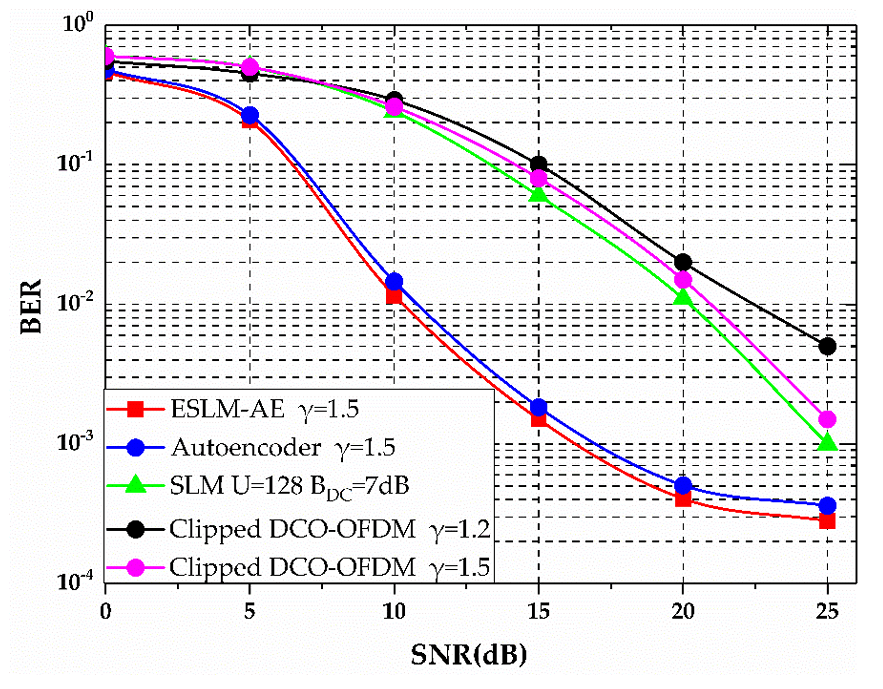
\includegraphics[width=\linewidth]{Figures/7.png}}
\caption{BER comparison of the clipped DCO-OFDM, SLM, Autoencoder and the proposed scheme under the DOW channel.}
\label{fig7}
\end{figure}

To demonstrate the influence of ISI, we set a shorter CP of 4-samples while the maximum delay of the multipath channel is 11. Fig.~\ref{fig8} gives the comparison of BER performance of the above methods in DOW channel with and without ISI. From the performance results, we can conclude that the ESLM-AE scheme outperforms conventional PAPR reduction methods in terms of both the BER and PAPR.

\begin{figure}[htbp]
\centerline{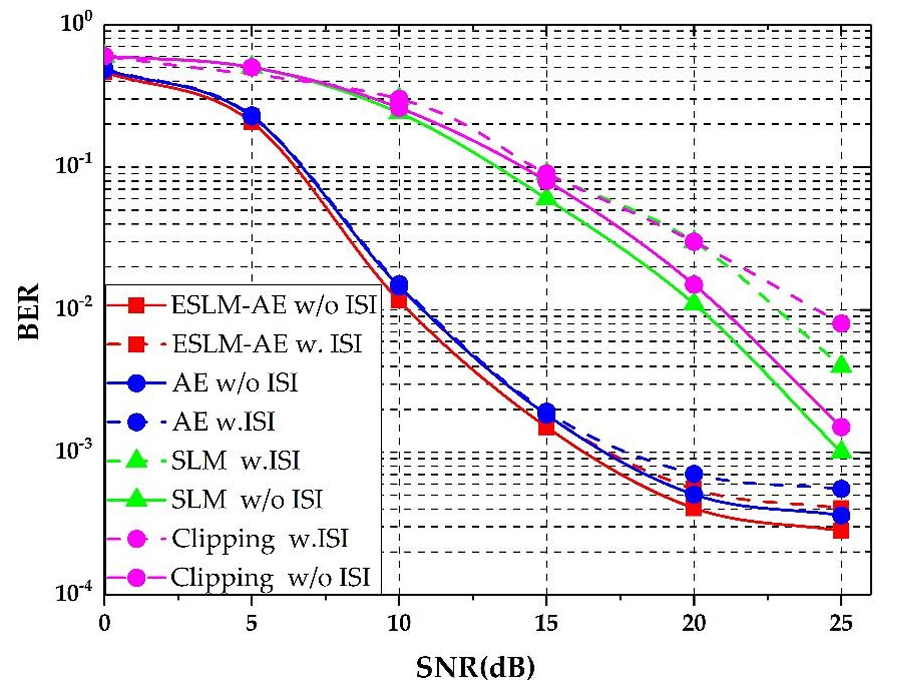
\includegraphics[width=\linewidth]{Figures/8.png}}
\caption{BER comparison of the clipped DCO-OFDM, SLM, Autoencoder and the proposed scheme under the DOW channel with/without ISI. The clipping ratios, $\gamma$, used for clipping, ESLM-AE and Autoencoder are 1.5.}
\label{fig8}
\end{figure}

\section{Conclusions}
This paper proposes an ESLM-AE network to reduce the PAPR value for the DCO-OFDM system without reducing the BER performance. The constellation mapping and de-mapping of the symbols and phase factor of each subcarrier are trained adaptively using a combined loss function of the AE with two different loss components. The simulation results show that our proposed scheme significantly outperforms conventional schemes in terms of both the PAPR and BER. By using our proposed technique, a distinct PAPR reduction of more than 10 dB is achieved for the VLC system, which significantly relieves the linear requirement of the front-end devices. Moreover, the decrease in the PAPR transforms to a BER performance gain both in the LOS channel and the DOW channel.

\begin{thebibliography}{00}

\bibitem{b1} Armstrong, J.; Schmidt, B.J. Comparison of asymmetrically clipped optical OFDM and DC-biased optical OFDM in AWGN. IEEE Commun. Lett. 2008, 12, 343--345.
\bibitem{b2} Komine, T.; Nakagawa, M. Fundamental analysis for visible-light communication system using LED lights. IEEE Trans. Consum. Electron. 2004, 50, 100--107.
\bibitem{b3} Lu, H.; Hong, Y.; Chen, L.-K.; Wang, J. On the study of the relation between linear/nonlinear PAPR reduction and transmission performance for OFDM-based VLC systems. Opt. Express 2018, 26, 13891--13901.
\bibitem{b4} Deng, L.; Fan, Y.; Zhao, Q. A novel PAPR reduction scheme for VLC DCO-OFDM systems. Opt. Commun. 2018, 426, 164--169.
\bibitem{b5} Singh, V.K.; Dalal, U.D. Abatement of PAPR for ACO-OFDM deployed in VLC systems by frequency modulation of the baseband signal forming a constant envelope. Opt. Commun. 2017, 393, 258--266.
\bibitem{b6} Vgenopoulou, V.; Song, M.; Pincemin, E.; Jaouën, Y.; Sygletos, S.; Roudas, I. Comparison of Nonlinear Compensation Techniques for 400-Gb/s Coherent Multi-Band OFDM Super-Channels. Appl. Sci. 2018, 8, 447.
\bibitem{b7} Tang, R.; Zhou, X.; Wang, C.; Haar, A. Wavelet Decision Feedback Channel Estimation Method in OFDM Systems. Appl. Sci. 2018, 8, 877.
\bibitem{b8} Goebel, B.; Hellerbrand, S.; Haufe, N.; Hanik, N. PAPR reduction techniques for coherent optical OFDM transmission. In Proceedings of the 11th International Conference on Transparent Optical Networks (ICTON'09), Azores, Portugal, 28 June--2 July 2009; pp. 1--4.
\bibitem{b9} Lu, H.; Zhang, L.; Wu, Z. Noise Resistant Spreading OOFDM Design for Suppressing PAPR of High Data Rate Wireless Optical Communication System. In Proceedings of the 2018 IEEE International Conference on Communications (ICC), Kansas City, MO, USA, 20--24 May 2018; pp. 1--6.
\bibitem{b10} Chronopoulos, S.K.; Christofilakis, V.; Tatsis, G.; Kostarakis, P. Reducing peak-to-average power ratio of a turbo coded OFDM. Wirel. Eng. Technol. 2012, 3, 195.
\bibitem{b11} Han, S.H.; Lee, J.H. PAPR reduction of OFDM signals using a reduced complexity PTS technique. IEEE Signal Process. Lett. 2004, 11, 887--890.
\bibitem{b12} Liu, Y.; Deng, H.; Ren, S.; Tang, C.; Qian, X. Peak-to-average power ratio reduction in orthogonal frequency division multiplexing-based visible light communication systems using a modified partial transmit sequence technique. Opt. Eng. 2018, 57, 016108.
\bibitem{b13} Zhang, H.; Yuan, Y.; Xu, W. PAPR reduction for DCO-OFDM visible light communications via semidefinite relaxation. IEEE Photonics Technol. Lett. 2014, 26, 1718--1721.
\bibitem{b14} Hei, Y.; Liu, J.; Li, W.; Xu, X.; Chen, R.T. Branch and bound methods based tone injection schemes for PAPR reduction of DCO-OFDM visible light communications. Opt. Express 2017, 25, 595--604.
\bibitem{b15} Hei, Y.; Liu, J.; Gu, H.; Li, W.; Xu, X.; Chen, R.T. Improved TKM-TR methods for PAPR reduction of DCO-OFDM visible light communications. Opt. Express 2017, 25, 24448--24458.
\bibitem{b16} Popoola, W.O.; Ghassemlooy, Z.; Stewart, B.G. Pilot-assisted PAPR reduction technique for optical OFDM communication systems. J. Lightw. Technol. 2014, 32, 1374--1382.
\bibitem{b17} Yu, B.; Zhang, H.; Wei, L.; Song, J. Subcarrier grouping OFDM for visible-light communication systems. IEEE Photonics J. 2015, 7, 1--12.
\bibitem{b18} Musumeci, F.; Rottondi, C.; Nag, A.; Macaluso, I.; Zibar, D.; Ruffini, M.; Tornatore, M. A Survey on Application of Machine Learning Techniques in Optical Networks. arXiv 2018, arXiv:1803.07976.
\bibitem{b19} O'Shea, T.J.; Hoydis, J. An introduction to machine learning communications systems. arXiv 2017, arXiv:1702.00832.
\bibitem{b20} Dörner, S.; Cammerer, S.; Hoydis, J.; ten Brink, S. Deep learning based communication over the air. IEEE J. Sel. Top. Signal Process. 2018, 12, 132--143.
\bibitem{b21} Ye, H.; Li, G.Y.; Juang, B.-H. Power of deep learning for channel estimation and signal detection in OFDM systems. IEEE Wirel. Commun. Lett. 2018, 7, 114--117.
\bibitem{b22} Kim, M.; Lee, W.; Cho, D.-H. A Novel PAPR Reduction Scheme for OFDM System Based on Deep Learning. IEEE Commun. Lett. 2018, 22, 510--513.
\bibitem{b23} O'Shea, T.J.; Karra, K.; Clancy, T.C. Learning to communicate: Channel auto-encoders, domain specific regularizers, and attention. In Proceedings of the 2016 IEEE International Symposium on Signal Processing and Information Technology (ISSPIT), Limassol, Cyprus, 12--14 December 2016; pp. 223--228.
\bibitem{b24} Felix, A.; Cammerer, S.; Dörner, S.; Hoydis, J.; ten Brink, S. OFDM-Autoencoder for End-to-End Learning of Communications Systems. arXiv 2018, arXiv:1803.05815.
\bibitem{b25} Sohn, I. A low complexity PAPR reduction scheme for OFDM systems via neural networks. IEEE Commun. Lett. 2014, 18, 225--228.
\bibitem{b26} Sohn, I.; Kim, S.C. Neural network based simplified clipping and filtering technique for PAPR reduction of OFDM signals. IEEE Commun. Lett. 2015, 19, 1438--1441.
\bibitem{b27} Csáji, B.C. Approximation with artificial neural networks. Fac. Sci. Etvs Lornd Univ. Hung. 2001, 24, 48.
\bibitem{b28} Hinton, G.E.; Salakhutdinov, R.R. Reducing the dimensionality of data with neural networks. Science 2006, 313, 504--507.
\bibitem{b29} Vaiyamalai, S.; Mahesula, S.; Dhamodharan, S.K. PAPR Reduction in SLM--OFDM System Using Lehmer Sequence Without Explicit Side Information. Wirel. Pers. Commun. 2017, 97, 5527--5542.
\bibitem{b30} Elgala, H.; Mesleh, R.; Haas, H. An LED model for intensity-modulated optical communication systems. IEEE Photonics Technol. Lett. 2010, 22, 835--837.
\bibitem{b31} Azim, A.W.; le Guennec, Y.; Maury, G. Decision-directed iterative methods for PAPR reduction in optical wireless OFDM systems. Opt. Commun. 2017, 389, 318--330.
\bibitem{b32} Ghassemlooy, Z.; Ma, C.; Guo, S. PAPR reduction scheme for ACO-OFDM based visible light communication systems. Opt. Commun. 2017, 383, 75--80.
\bibitem{b33} O'Shea, T.; Hoydis, J. An introduction to deep learning for the physical layer. IEEE Trans. Cogn. Commun. Netw. 2017, 3, 563--575.
\bibitem{b34} Ito, Y. Representation of functions by superpositions of a step or sigmoid function and their applications to neural network theory. Neural Netw. 1991, 4, 385--394.
\bibitem{b35} Srivastava, N.; Hinton, G.; Krizhevsky, A.; Sutskever, I.; Salakhutdinov, R. Dropout: A simple way to prevent neural networks from overfitting. J. Mach. Learn. Res. 2014, 15, 1929--1958.
\bibitem{b36} Ta\c{s}pınar, N.; Yıldırım, M. A novel parallel artificial bee colony algorithm and its PAPR reduction performance using SLM scheme in OFDM and MIMO-OFDM systems. IEEE Commun. Lett. 2015, 19, 1830--1833.
\bibitem{b37} Yuan, J.-G.; Shen, Q.; Wang, J.-X.; Wang, Y.; Lin, J.-Z.; Pang, Y. A novel improved SLM scheme of the PAPR reduction technology in CO-OFDM systems. Optoelectron. Lett. 2017, 13, 138--142.
\bibitem{b38} Chronopoulos, S.K.; Tatsis, G.; Raptis, V.; Kostarakis, P. Enhanced PAPR in OFDM without deteriorating BER performance. Int. J. Commun. Netw. Syst. Sci. 2011, 4, 164.
\bibitem{b39} Goodfellow, I.; Bengio, Y.; Courville, A.; Bengio, Y. Deep Learning; MIT Press: Cambridge, MA, USA, 2016.
\bibitem{b40} Nair, V.; Hinton, G.E. Rectified linear units improve restricted boltzmann machines. In Proceedings of the 27th International Conference on Machine Learning (ICML-10), Haifa, Israel, 21--24 June 2010; pp. 807--814.
\bibitem{b41} Hu, W.-W.; Lee, D.-H. PAPR Reduction for Visible Light Communication Systems Without Side Information. IEEE Photonics J. 2017, 9, 1--11.
\bibitem{b42} Chronopoulos, S.K.; Christofilakis, V.; Tatsis, G.; Kostarakis, P. Preliminary BER study of a TC-OFDM system operating under noisy conditions. J. Eng. Sci. Technol. Rev. 2016, 9, 13--16.
\bibitem{b43} Yang, B.; Letaief, K.B.; Cheng, R.S.; Cao, Z. Channel estimation for OFDM transmission in multipath fading channels based on parametric channel modeling. IEEE Trans. Commun. 2001, 49, 467--479.
\bibitem{b44} Chy, D.K.; Khaliluzzaman, M. Evaluation of SNR for AWGN Rayleigh and Rician Fading Channels Under DPSK Modulation Scheme with Constant BER. Int. J. Wirel. Commun. Mob. Comput. 2015, 3, 7--12.
\bibitem{b45} Ndjiongue, A.R.; Ngatched, T.M.; Ferreira, H.C. On the Indoor VLC Link Evaluation Based on the Rician K-Factor. IEEE Commun. Lett. 2018, 22, 2254--2257.
\bibitem{b46} Wilson, S.K.; Holliday, J. Scheduling methods for multi-user optical wireless asymmetrically-clipped OFDM. J. Commun. Netw. 2011, 13, 655--663.
\bibitem{b47} Carruthers, J.B.; Kahn, J.M. Modeling of nondirected wireless infrared channels. IEEE Trans. Commun. 1997, 45, 1260--1268.

\end{thebibliography}

\end{document}
